\section{Informatique contextuelle}\label{sec:rw:supervision:contexte}
Au centre des systèmes pervasifs et de l'informatique ubiquitaire, l'informatique contextuelle prend une importance de plus en plus grande. Sa définition a fait l'objet de plusieurs débats au sein de la communauté scientifique. La définition la plus couramment utilisée est : \enquote{L'informatique contextuelle (\textit{context-aware computing} a pour but de permettre aux équipements de fournir de meilleurs services aux utilisateurs par l'utilisation d'informations de contexte}\cite{Han:contextaware}. Ainsi, le point important est de former un ensemble d'information pour que des applications puissent adapter leur fonctionnement. L'instanciation de cette notion de contexte est un processus d'observation de l'environnement dans lequel se trouve l'application.

La section~\ref{sec:rw:supervision:administration} a permis de voir que le système observé peut fournir de grandes quantités de données. Grâce à l'informatique contextuelle, nous souhaitons pouvoir donner de la cohérence à ces données. Ainsi, nous pouvons mieux exploiter leur sémantique et envisager d'effectuer de l'observation de plus haut niveau afin d'établir un diagnostic.

Cette section présente d'abord les définitions et applications de l'informatique contextuelle. Par la suite, nous détaillons la façon dont le contexte est capturé et modélisé. Nous présentons les capacités de traitement sur celui-ci. Enfin, nous analysons différents systèmes pervasifs afin de percevoir la mise en application de cette approche. Nous concluons par une synthèse, détaillant l'adéquation aux critères de notre problématique.

\subsection{Définitions et applications}
La définition de contexte a été elle aussi au cœur de nombreux débats. Après analyse des travaux sur le sujet, le rapport de recherche~\cite{Dey:context} propose la définition suivante : \enquote{\it Un contexte est toute information pouvant être utilisée pour caractériser la situation d'une entité. Cette entité pouvant être une personne, un lieu, ou un objet considéré comme pertinent à l'interaction entre l'utilisateur et le système.}.

Il est important de noter que cette définition est orientée par l'utilisation qui en est faite. Une donnée quelconque peut faire partie d'un contexte si elle est utilisée comme tel. Ainsi, il est nécessaire de voir l'ensemble des utilisations de ce contexte. Celles-ci sont rassemblées dans sept catégories principales~\cite{Soylu:context} : 
\begin{enumerate}
	\item Sélection et recommandations d'informations ou de services.
	\item Présentation et accès à l'information et aux services.
	\item Recherche d'information ou de service.
	\item Adaptation de l'exécution de processus séquentiels.
	\item Modification et reconfiguration d'applications.
	\item Conseil d'actions semi-automatique.
	\item Allocations de ressources.
\end{enumerate}
Les utilisations du contexte sont directement reliées à l'observation, car c'est elle qui permet la construction du contexte.

\subsection{Modélisation et capture du contexte}
Le modèle utilisé pour créer et manipuler le contexte peut être de différentes formes : basé sur des principes d'intelligence artificielle (représentations de connaissances, réseaux bayésiens), le génie logiciel (UML), les bases de données (ER : Entité-Relation) ou d'autres moyens applicatifs (arbres, entrées clefs-valeurs). L'UML et l'ER atteignent rapidement leurs limites d'expressivité. Il devient difficile de manipuler les données dans le cadre de contextes larges et hétérogènes à cause de leur rigidité. Ces modèles permettent d'abstraire une partie du monde ou de la logique pour un usage restreint. Par opposition, la gestion de données issues d'ontologies est moins soumise à cette rigidité.

\subsubsection{Un modèle sous forme de triplet}
Pour représenter l'ensemble des connaissances sur le système, autant en terme de structure que de données, les contextes sont la plupart du temps modélisés comme un réseau sémantique. Le langage communément utilisé pour cela est le RDF (\textit{Resource Description Framework})~\cite{W3C:RDF}, un standard répandu. Son principe est à la fois simple et puissant. Son expression est simple, car toute sa structure est orchestrée par des triplets : Objet, Relation, Valeur. Par exemple, \textit{la télévision} \textbf{est située dans} \textit{le salon}. De même, \textit{le salon} \textbf{est une} \textit{pièce}. L'ensemble des triplets forme un graphe où les objets et valeurs sont des nœuds et les relations sont des liens, d'où l'appellation de \textit{graphe sémantique}~\cite{Minsky:knowledge}. Pour étendre l'expressivité des graphes sémantiques et y apporter la notion de classes, les ontologies se sont développées.

\subsubsection{Les ontologies}
Tel que l'a défini Kalfoglou~\cite{Kalfoglou:ontology}, une ontologie est \textit{une représentation explicite d'une compréhension commune de concepts importants appartenant à un domaine d'intérêt}.
Elle permet de capturer et de représenter une vue simplifiée d'un domaine à travers des concepts prédéfinis. Cela permet un langage commun et une taxonomie des concepts, mais aussi, l'ontologie est capable de représenter leurs liaisons. Ainsi, il est possible de modéliser la sémantique propre des différentes données.

Les ontologies sont toutefois structurées dans un langage qui permet de définir les grandes catégories de relations ou d'objets. Plusieurs langages existent, mais tous définissent les entités suivantes :
\begin{itemize}
    \item[\textbf{Concepts}] Décrivent les classes et sous-classes de toutes les choses du monde.
    \item[\textbf{Instances}] Ce sont les individus correspondant aux concepts.
    \item[\textbf{Relations}] Permet de lier les concepts et instances entre eux. Une des relations principales est la relation \textit{Est-Un} (\textit{Is-A} en anglais) qui lie une instance à un concept.
    \item[\textbf{Types de données}] Types syntaxique d'une donnée : entier, chaîne de caractères, booléen.
    \item[\textbf{Valeurs}] Valeur qu'un concept ou instance peut avoir.
\end{itemize}

Par la suite, les langages permettent différentes manières de lier les concepts entre eux. Cette capacité va permettre de montrer l'expressivité de la structure. Par exemple, une des relations des plus importantes est la relation de hiérarchie. Un \textit{chien} \underline{est une sous-classe d}'\textit{animal}, et \textit{labrador} \underline{est une sous-classe de} \textit{chien}. La \textit{relation de hiérarchie} \underline{est une} \textit{relation transitive}. Ainsi, le langage vérifie naturellement que le \textit{labrador} \underline{est une sous-classe d}'\textit{animal}. 

La logique permettant d'exprimer ces contraintes et inférences structurelles est une logique de description. Suivant la classe de la logique de description sous-jacente, le langage est plus ou moins complexe à traiter par la suite\footnote{Dans certains cas, comme OWL-Full, son expressivité est tellement large qu'il devient indécidable de vérifier si un concept appartient à une classe.}. Par exemple, le langage le plus utilisé reste \textit{OWL Lite}, équivalent à la logique $\mathcal{SHIF}^\mathcal{(D)}$. Cette logique permet lors de la description des concepts l'utilisation des constructeurs suivants : quantification universelle, négation\footnote{Si la négation et la quantification universelle existent, alors le prédicat d'existence est autorisé, car $\not\forall \equiv \exists$}, transitivité de relation, inversion de relation, hiérarchie de relations. De plus, l'usage de propriétés fonctionnelles et de données est possible. En revanche, la restriction d'une collection à un nombre d'éléments donné par exemple n'est pas possible. Son utilisation est répandue, car les inférences sont calculables dans la pratique contrairement à des logiques plus expressives.

Comparées à des structures telles qu'UML, les ontologies jouissent de la flexibilité des réseaux sémantiques. Il est toutefois important de noter que cette puissance et cette liberté rendent sa manipulation délicate. En effet, il est supposé que toutes les sources de connaissances s'appuient sur une ontologie commune. Il est important d'être minutieux dans la manipulation de cette structure pour éviter par exemple des duplications de concepts, voire des conflits de définitions.

\subsubsection{Capture du contexte}
La capture du contexte est la manière de récupérer une information et de la représenter sous la forme choisie lors de la modélisation. Par exemple, un capteur de température peut insérer un ensemble de triplets pour indiquer qu'à 10h25 le lundi 26 avril, il faisait 25.256ºC sur la source T75896. Cet ensemble de triplets dépend de la modélisation des concepts qui forme le contexte. Lors de la capture, les données sont issues du système observé ou par l'extraction de nouvelles connaissances construites à partir d'informations déjà capturées.

La gestion de l'hétérogénéité est rarement mentionnée puisque les sources de données sont censées être conformes au schéma commun. Toutefois, comme présenté dans~\cite{Kaed:these}, il est possible d'aligner les modèles des sources avec un schéma commun. Le formalisme des ontologies permet en effet de décrire les équivalences logiques entre différents concepts ce qui permet l'intégration de données.

\subsection{Capacités de traitement}
Un intérêt des réseaux sémantiques est le pouvoir de raisonnement logique. Le but ici est de pouvoir inférer de nouveaux triplets à partir des connaissances accumulées. Pour cela, il existe plusieurs langages permettant de spécifier ces inférences. Le plus courant est le langage associé à \textit{RDF} : \textit{SPARQL}. Ce langage a la particularité d'être aussi expressif que l'algèbre relationnelle~\cite{Angles:sparql}\footnote{Plus exactement, SparQL est équivalent au \textit{datalog} non récursif avec négation, ce qui est équivalent à l'algèbre relationnelle.}. Ainsi, il est possible de faire des inférences du premier ordre sur ces données.

Ces inférences sont de trois types :
\begin{itemize}
 \item[\textbf{Association directe}] Une information bas-niveau est associée à une information haut-niveau 
 \item[\textbf{Fusion de contexte}] Un ensemble de données infère un nouvel état 
 \item[\textbf{Fission de contexte}] Une donnée infère un ensemble d'informations
\end{itemize}

Dans l'informatique contextuelle, il est important de distinguer plusieurs espaces de données~\cite{Padovitz:agent} :
\begin{itemize}
 \item[\textbf{L'espace de valeur}] Par exemple, pour une personne, son age est compris entre 0 et 125.
 \item[\textbf{L'espace applicatif}] L'ensemble des données atomiques qui représentent le contexte dit de bas-niveau.
 \item[\textbf{L'espace de situation}] Reflète les situations pouvant être extraites de l'espace applicatif.
\end{itemize}

À un instant donné, il est possible de définir un \textbf{état de contexte} en tant que collection d'attributs de l'espace de contexte. Cet état peut par la suite inférer un ensemble de situations. La figure~\ref{rw-supervision-contextreasoning} résume la structure abstraite du raisonnement sur les contextes.

\begin{figure}[ht]
    \centering
    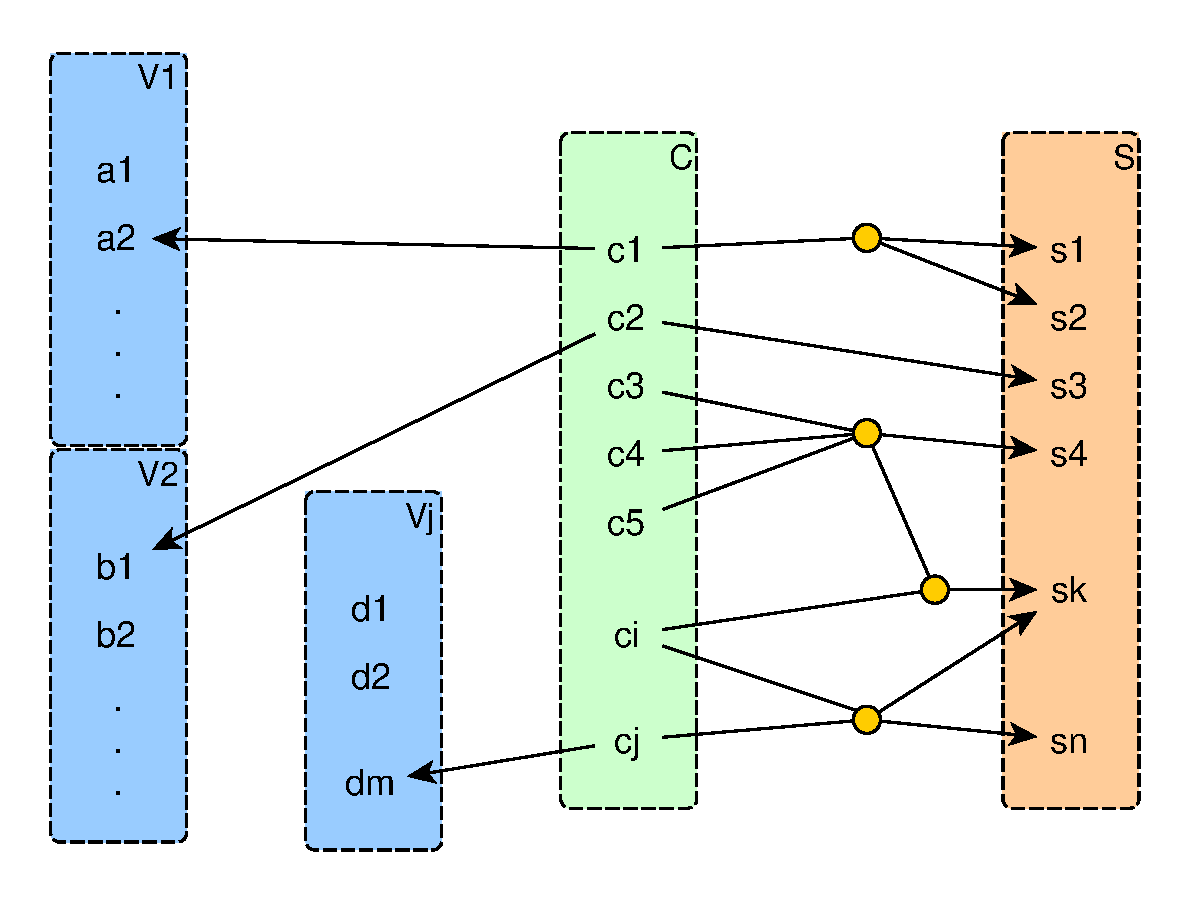
\includegraphics[width=.50\textwidth]{rw-supervision-contextreasoning}
    \caption{Structure abstraite du raisonnement sur contexte. À un élément du contexte $c_i$ est associée une valeur du domaine $V_i$. À partir de l'espace du contexte $C$, on effectue des associations, des fissions ou fusions pour inférer l'espace des situations $S$.}\label{rw-supervision-contextreasoning}
\end{figure}

\subsubsection{La qualité de contexte}
La qualité du contexte~\cite{Buchholz:quality} est définie comme toute information permettant de décrire la qualité des informations contenues dans le contexte. Le point crucial est que cette qualité n'est pas liée à un quelconque processus ou matériel. Elle peut se décliner en plusieurs \textit{paramètres} : précision, fiabilité, confiance, fraicheur,\dots{}

La qualité des données a des impacts lors du diagnostic. Supposons que nous constatons un problème de pixélisation TV. Cette situation a été inférée par la valeur actuelle d'une métrique indiquant le nombre d'images non décodées. Premièrement, si la source de donnée remontant la métrique n'est pas assez fiable, nous pouvons mettre en doute les relevés. De plus, il est possible que l'information ne reflète pas l'état actuel. Ainsi, la situation indiquant un problème est vraie à la qualité des sources près.

De plus, si nous souhaitons effectuer un diagnostic, nous pouvons indiquer au système que ce type de panne est dû à un problème de lenteur de réseau interne. Toutefois, ce peut être dû à des dysfonctionnements plus rares, comme une panne matérielle. Ainsi, certaines recherches permettent d'introduire une part de probabilités dans les raisonnements pourtant déterministes a priori~\cite{Padovitz:agent}.

Dans cette thèse, nous ne détaillons pas le concept de qualité des données. Néanmoins, nous pouvons voir que cela peut avoir des impacts majeurs. L'utilisation de ces travaux serait intéressant pour des améliorations futures.

\subsection{Analyse de systèmes d'observation à base de contextes existants}
Dans cette partie, nous analysons des systèmes pervasifs à base de contexte existant. Ceux-ci sont en général très utilisés dans le réseau domestique qui est l'environnement de développement le plus courant dans le domaine de l'informatique ubiquitaire. Cette étude nous permet de voir comment est mise en pratique l'approche présentée jusqu'ici.

\subsubsection{De la représentation du système}
\textit{DogOnt}~\cite{Bonino:dogont}, a pour objectif de pouvoir modéliser les objets des environnements domotiques intelligents. Ainsi, en plongeant l'ensemble des équipements au niveau conceptuel des ontologies, il est possible de résoudre les problèmes d'interopérabilité et d'hétérogénéité des données. \textit{DogOnt} est capable de répondre à des requêtes telles que : la position de l'équipement, ses capacités, ses moyens de communication, comment l'environnement est composé (notamment architecturalement parlant, ce qui permet de représenter la maison).

Ainsi, une représentation de haut niveau permet de poser tous les concepts afin de représenter le réseau domestique au sens large. D'une manière plus concrète, un équipement est représenté en tant que \enquote{\it Controllable} (et ses sous-classes). Cette ontologie est représentée dans la figure~\ref{fig:rw:supervision:dogont}.

\begin{figure}[ht]
    \centering
    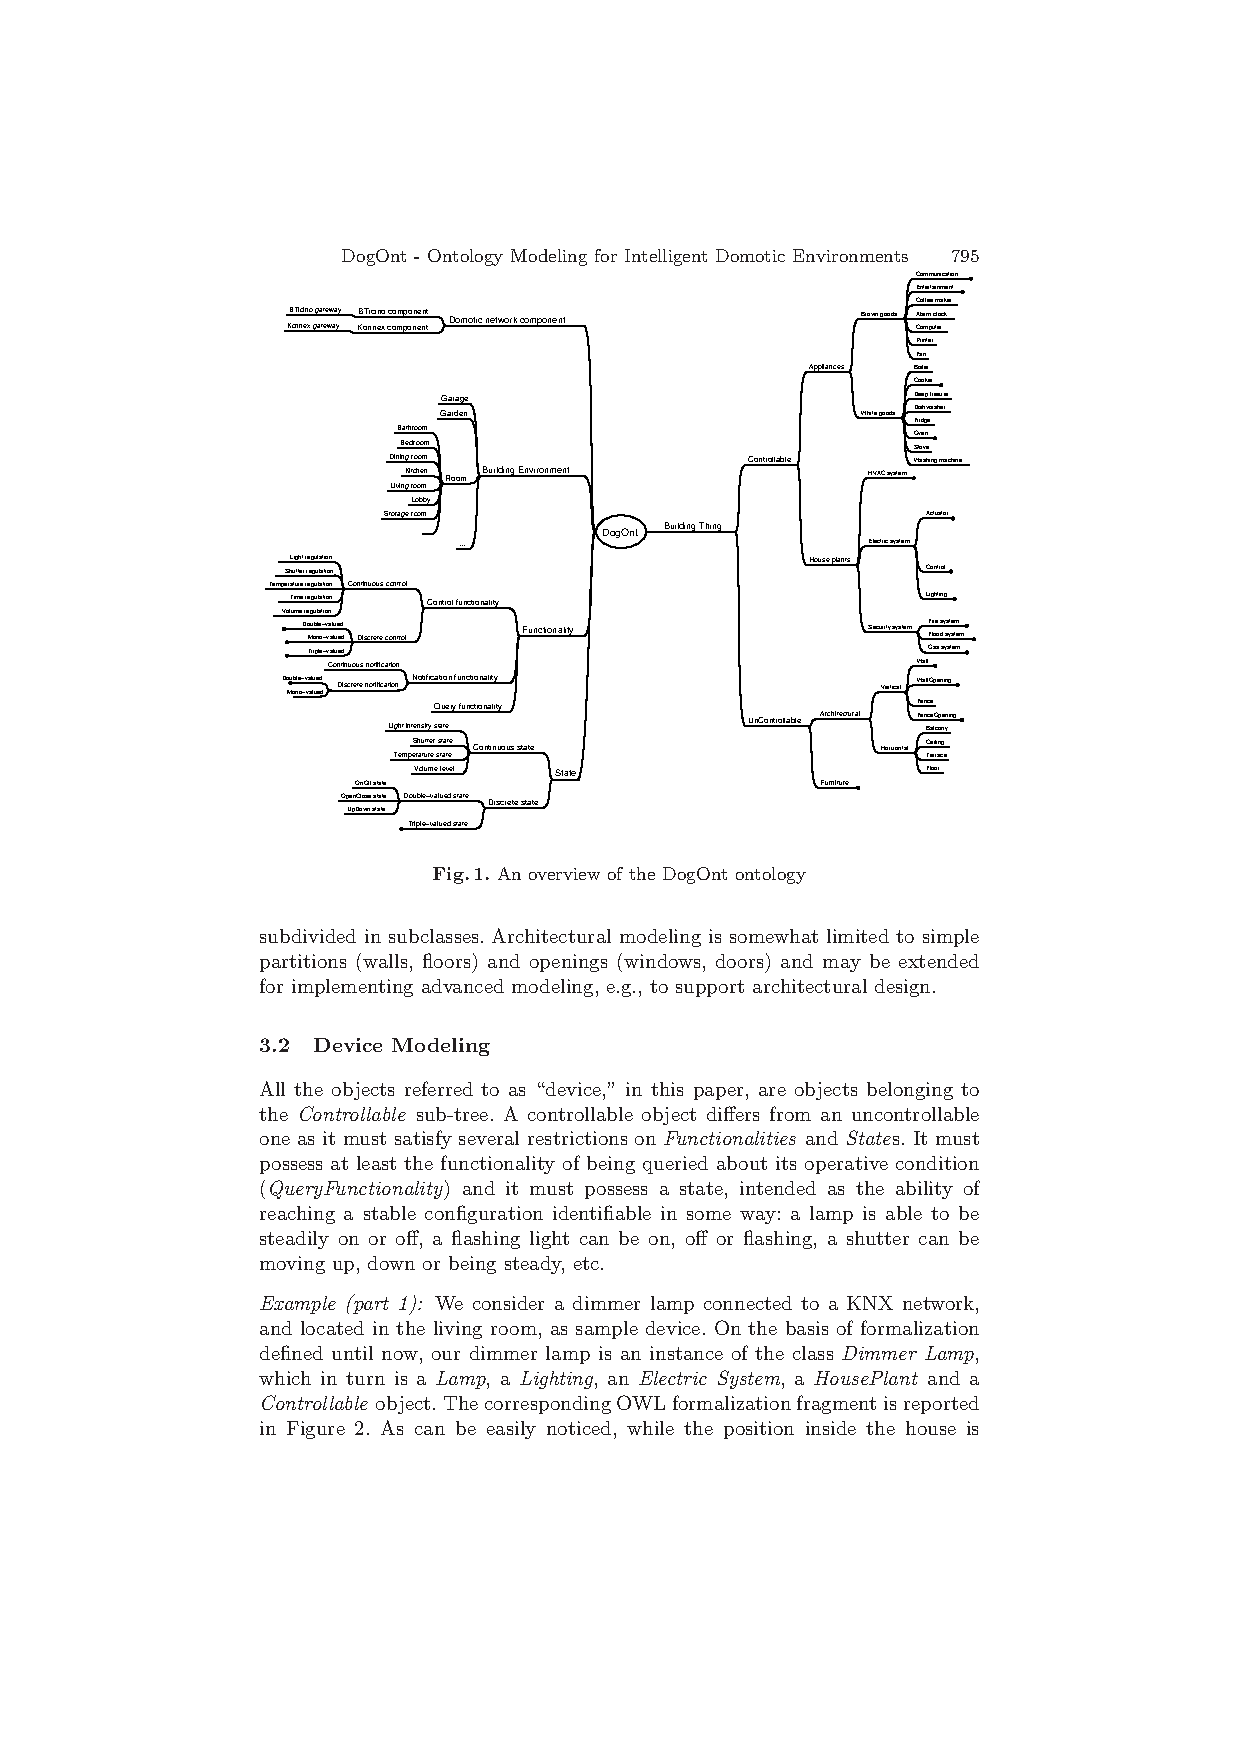
\includegraphics[width=0.8\textwidth, trim=4cm 15.5cm 4cm 4.6cm, clip]{rw-supervision-dogont}
    \caption{L'ontologie de DogOnt}\label{fig:rw:supervision:dogont}
\end{figure}
Pour pouvoir observer, et contrôler, les instances de ces concepts, il est nécessaire de rajouter des fonctionnalités et des variables d'états. Ceci se fait par l'introduction de relations sémantiques telles que \textit{hasControl}, \textit{hasFunctionality}, et \textit{hasState}. En combinant ces associations ainsi que l'ensemble complet des instances, il est possible de représenter l'ensemble des périphériques et leurs capacités.

Plusieurs autres projets ont utilisé ce type de modélisation pour des applications pervasives. Par exemple, Amigo~\cite{BenMokhtar:easy} se focalise plus sur la modélisation des services et des capacités. A contrario, \textit{MATCH}~\cite{Docherty:match} met l'accent sur la hiérarchie des ontologies pour que chaque domaine puisse apporter ses connaissances en utilisant des concepts communs (\textit{dispositifs}, \textit{réseau},\dots).

Nous remarquons que la séparation des domaines permet de gérer les perspectives utilisateurs en fonction de leurs intérêts. De plus, nous notons que l'hétérogénéité des schémas conceptuels est gérée par l'utilisation d'une ontologie commune. La nécessité d'une ontologie commune est récurrente dans ces travaux. Toutefois, dans des travaux récents~\cite{Niang:global,Niang:integration}, il existe des approches semi-automatiques pour intégrer des données de sources hétérogènes via la génération d'une ontologie commune et d'alignements.

\subsubsection{SOCAM : De l'utilité du raisonnement logique}
SOCAM (Service-Oriented Context-Aware Middleware)~\cite{Gu:socam} propose un intergiciel générique pour permettre aux développeurs de créer des applications pervasives par contexte. Cet intergiciel supporte l'acquisition, la découverte, l'interprétation et l'accès aux contextes. Comme les autres solutions présentées jusqu'ici, il s'appuie sur une ontologie conceptualisée comme celle de \textit{MATCH} afin de pouvoir être générique et y apporter les connaissances de chacun des domaines.

L'architecture de SOCAM, représentée en figure~\ref{fig:rw:supervision:socam} qui se décrit en trois 4 composants principaux.
\begin{figure}[ht]
    \centering
    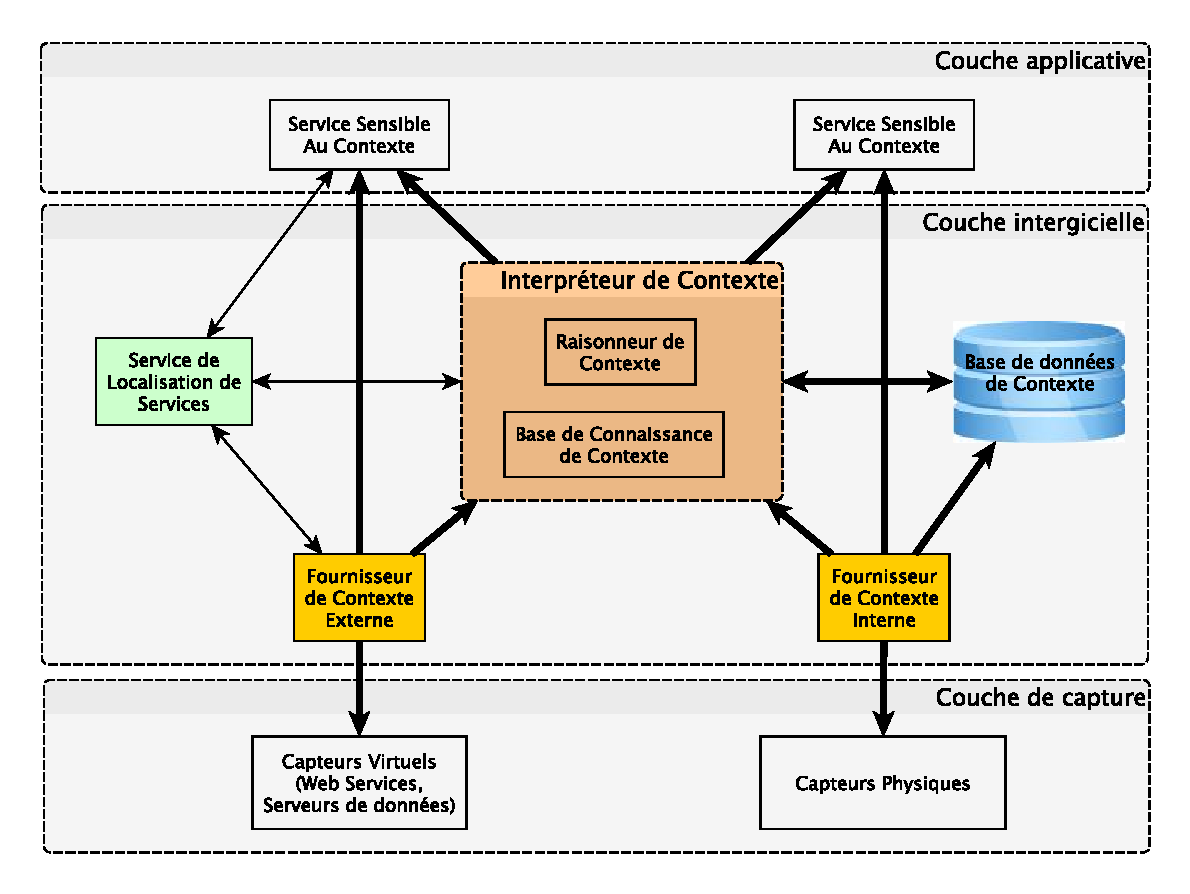
\includegraphics[width=0.66\textwidth]{rw-supervision-socam}
    \caption{Architecture de SOCAM}\label{fig:rw:supervision:socam}
\end{figure}
\begin{itemize}
	\item[\textbf{Fournisseurs de contexte}] Qui permet d'abstraire l'hétérogénéité des données issues des différentes sources (internes, tels que les capteurs ou autres dispositifs), ou externe (services météo ou autres) pour les convertir en \textit{OWL}.
    \item[\textbf{Interpréteur de contexte}] Fournit la logique de raisonnement sur le contexte.
    \item[\textbf{Base de données de contexte}] Stocke les ontologies de contexte et l'historique des contextes pour chaque sous-domaine.
    \item[\textbf{Service de localisation de services}] Sert de catalogue des services externes disponibles. Sa sélection peut se faire sur un type de service, mais il peut aussi faire une comparaison sur le contexte que le service fournit.
\end{itemize}
Les services applicatifs utilisant la notion de contexte vont ainsi utiliser les fonctionnalités que fournit SOCAM pour gérer cet ensemble de données. Une manière classique de construire ces services est de spécifier des actions déclenchées par un ensemble de règles au moment où le contexte change.

SOCAM implémente deux manières de faire de l'inférence logique de prédicats. La première est l'inférence structurelle. En effet, l'application d'une propriété transitive à un concept nous donne plusieurs informations. Par exemple, nous pouvons inférer que l'appareil \textit{Livebox} est une passerelle internet. Or, tous les équipements de cette catégorie ont des propriétés telles que la capabilité à gérer les règles de routage. La deuxième manière d'inférer des informations est un ensemble de règles utilisateurs. En utilisant un moteur similaire aux moteurs \textit{Prolog}, il est possible d'induire des informations qui constituent l'ensemble des situations. Par exemple, les auteurs présentent l'inférence du triplet \textit{(user socam:status 'SLEEPING')} par la détection de la position allongée dans la chambre avec la lumière éteinte.

Nous remarquons ici la présence d'une couche de traitement de données entre les sources et les services qui les utilisent. Cette couche se base sur des inférences logiques qui utilisent un support persistant pour constituer son contexte.

\subsection{Synthèse}
En conclusion, le traitement contextuel des données permet de gérer l'hétérogénéité sémantique des données. Les capacités de traitements sont liées à l'inférence logique pour enrichir la base des connaissances accumulées. Ainsi, il est possible de construire un espace de contexte et d'en inférer des situations de haut niveau. Cette capacité d'abstraction est nécessaire pour l'informatique ubiquitaire qui a besoin de manipuler des concepts humains.

Pour notre problématique d'observation, il reste difficile de gérer l'évolution des données au cours du temps. La liberté d'expression des bases de connaissances fait que l'inférence est complexe à manipuler. Plusieurs travaux s'attellent à permettre aux connaissances et aux règles d'introduire la dimension dynamique~\cite{Weikum:webknowledge, Hellerstein:declarative}. L'apport de cette dimension est toutefois difficile d'un point de vue théorique.

\begin{table}[!ht]
\criteretabDonnee
    {Structure sémantique à base de triplet.}
    {Utilisation d'ontologies. Gestion des contraintes et de l'inférence structurelles variable suivant l'expressivité du langage. En général, \textit{OWL Lite} est utilisé.}
    {Pas de gestion explicite du dynamisme en dehors d'annotations.}
\criteretabTraitement
    {Instantané uniquement.}
    {Les sources s'intègrent en se conformant à un modèle commun. Si tel n'est pas le cas de façon native, des règles d'alignements d'ontologies sont à fournir.}
    {Paradigme déclaratif en général dérivé de programmation logique allant de \textit{Prolog} à \textit{SPARQL}.}
    {Cela part de la logique du premier ordre complète à la capacité de l'algèbre relationnelle (\textit{datalog} non récursif avec négation)}
\criteretabAdaptabilite
    {Nécessité de spécifier des ontologies de domaines pour donner la structure des concepts du système.}
    {La séparation des domaines et le rattachement des données aux domaines permettent de clairement spécifier les différentes perspectives.}
    {Pas d'extensibilité possible sur le traitement d'inférence. Par contre, il est possible suivant l'architecture du système final de créer des capteurs de contextes pour fournir des données logiques de haut niveau.}
    {La complexité de l'inférence peut aller jusqu'en \textit{EXPTIME}. Toutefois, plusieurs implémentations optimisées permettent de traiter des millions de triplets en quelques secondes.}
\caption{Synthèse de l'informatique contextuelle}\label{tab:rw:supervision:contexte:synthese}
\end{table}
